\chapter{Estudo de Caso}
Este capítulo apresenta o estudo de caso conduzido com professores de \textit{introdução à programação} com o objetivo de investigar a viabilidade, utilidade prática e os desafios associados ao uso de templates multicamadas proposto neste trabalho. A pesquisa adota uma abordagem integrada à pesquisa-ação, com uso de métodos mistos (quantitativos e qualitativos). O estudo foi conduzido e estruturado para oferecer evidências que respondem às três questões de pesquisa (QP1, QP2 e QP3) conforme as diretrizes metodológicas recomendadas pela \gls{ceie} para estudos de caso.

\section{Objetivo do Estudo}
O objetivo deste estudo de caso é investigar a aplicabilidade da geração automática de questões utilizando templates multicamadas no contexto do ensino de programação, com base na experiência de professores na construção desses templates, e em suas percepções sobre a utilidade e os desafios da abordagem. Para isso, são apresentados a abordagem utilizada,  os procedimentos envolvidos e as métricas adotadas, que fundamentam a coleta e análise dos dados que serão discutidos nas seções seguintes.
Embora não tenha sido possível aplicar o feedback automatizado aos participantes devido ao tempo limitado para o desenvolvimento deste estudo, a literatura  indica que este recurso tem potencial significativo para contribuir no aprendizado, como evidenciado por trabalhos como o de \parencite{vanpraet2024} e \parencite{fung2024} indicam que a incorporação de feedback automatizado se utilizado corretamente pode aumentar de forma significativa o desempenho dos estudantes.

\section{Metodologia do Estudo de Caso}

Este estudo adotou uma abordagem mista que combina técnicas quantitativas e qualitativas dentro de um ciclo de pesquisa. A opção por integrar essas abordagens decorreu de duas necessidades complementares: mensurar, de forma objetiva, o tempo gasto, o número de questões produzidas e a taxa de reaproveitamento dos \textit{templates}, ao mesmo tempo em que se investigavam as percepções, dificuldades e sugestões dos professores.


\subsection{Perfil dos Professores}
Para garantir que os resultados reflitam um panorama representativo dos professores de Introdução a programação, foi definido dois critérios de inclusão e coleta de informação para cada professor com base nos seguintes aspectos: 

\begin{itemize}
    \item \textbf{Experiência recente}: lecionam ou lecionaram disciplinas introdutórias de programação em pelo menos 2 semestres nos cinco anos anteriores ao estudo.
    \item \textbf{Disponibilidade}: Compromisso para criar e avaliar templates e responder o questionário.
\end{itemize}

As Figuras \ref{fig:nivel-escolaridade}, \ref{fig:anos-docencia} e \ref{fig:linguagens-ensinadas} apresentam respectivamente, a distribuição dos participantes em relação ao nível de escolaridade, aos anos de experiência docente e às linguagens de programação ensinadas.

\begin{figure}[ht]
	\centering
	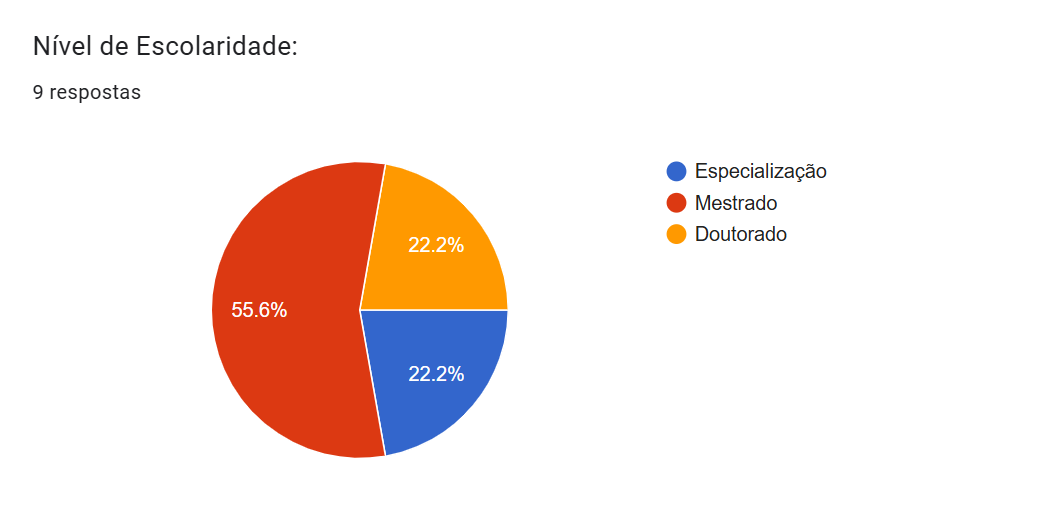
\includegraphics[width=18cm]{./imagens/capitulo8/1-escolaridade}
	\caption{Perfil Profissional 1 (Elaboração própria, 2025) }
	\label{fig:nivel-escolaridade}
\end{figure}
\begin{figure}[ht]
	\centering
	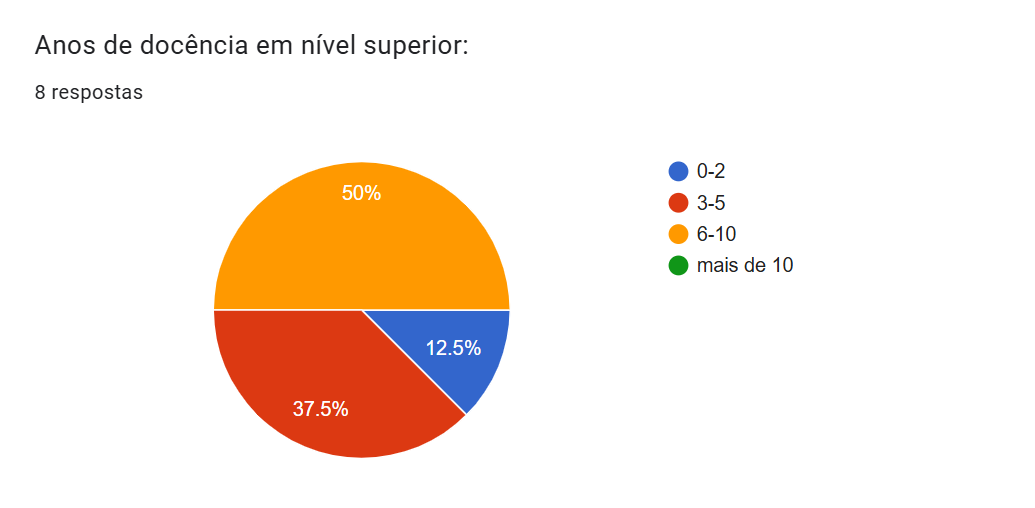
\includegraphics[width=18cm]{./imagens/capitulo8/2-anos-docencia}
	\caption{Perfil Profissional 2 (Elaboração própria, 2025) }
	\label{fig:anos-docencia}
\end{figure}
\begin{figure}[ht]
	\centering
	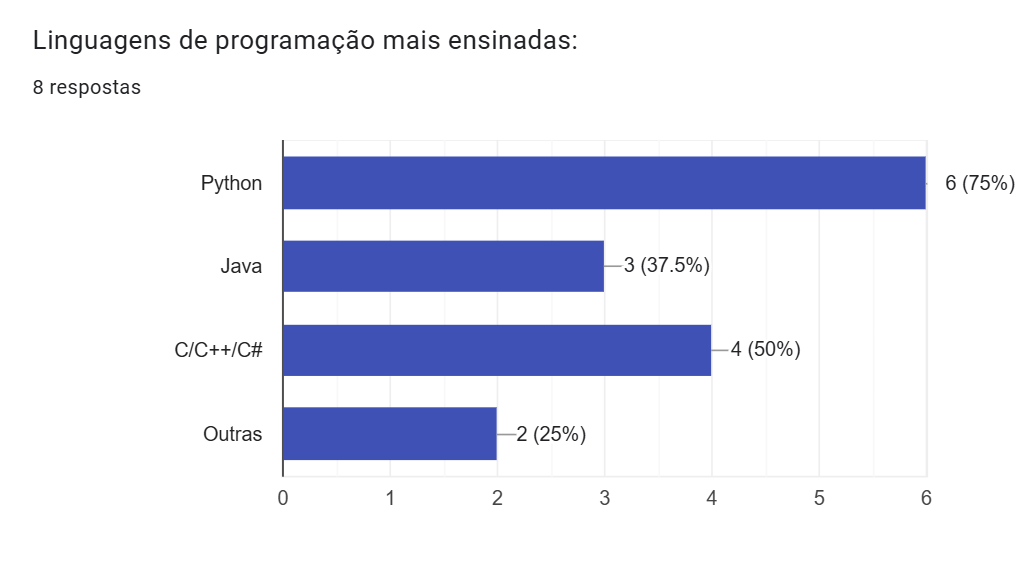
\includegraphics[width=18cm]{./imagens/capitulo8/2-linguagens-ensinadas}
	\caption{Perfil Profissional 3 (Elaboração própria, 2025) }
	\label{fig:linguagens-ensinadas}
\end{figure}

 
\subsection{Variáveis levantadas pelo questionário}
O formulário (ver Apêndice 1) foi dividido em 4 blocos, cada um mapeando uma das questões de pesquisa:

\begin{table}[H]
    \centering
    \begin{tabular}{|p{4cm}|p{5.4cm}|p{6cm}|}
        \hline
        \textbf{Bloco} & \textbf{Variáveis coletadas} & \textbf{Objetivo} \\ \hline
        Perfil profissional & Titulação, anos de docência, linguagens mais ensinadas. & Relacionar experiência ao \textbf{tempo médio} de criação de templates. \\ \hline
        Prática com templates & Tempo gasto, número de questões geradas, taxa de reaproveitamento. & Medir \textbf{viabilidade} e \textbf{utilidade} operacional. \\ \hline
        Percepções e desafios & Dificuldades encontradas, contribuição percebida, preferências de uso. & Identificar \textbf{barreiras} técnicas e pedagógicas. \\ \hline
        Adaptação de questões existentes & Grau de facilidade em converter questões próprias para o formato multicamada. & Verificar \textbf{capacidade de transformação} sem suporte externo. \\ \hline
    \end{tabular}
    \caption{Estrutura do questionário (Elaboração própria, 2025)}
    \label{tab:questionario-objetivos}
\end{table}

\subsection*{Etapas do Estudo}

O processo metodológico foi dividido em cinco etapas com o intuito de captar as percepções subjetivas dos professores:

\begin{enumerate}
    \item \textbf{Apresentação da proposta}: Foi exibido um vídeo curto dividido em três blocos (direcionamento, questões base e estrutura do modelo) com explicações sobre os fundamentos da geração automática de questões usando templates multicamadas, além de orientações de uso e exemplos práticos. O objetivo foi garantir a compreensão do assunto por parte dos professores.

    \item \textbf{Criação de templates pelos professores}: Após a apresentação do modelo, os professores elaboraram templates utilizando uma estrutura previamente definida. A orientação fornecida foi dividida em três tópicos principais:
    \begin{itemize}
        \item \textbf{Direcionamento}: Fundamentos e exemplos com perguntas-chave para ajudar na formulação do enunciado e identificação dos elementos variáveis.
        \item \textbf{Questões base}: Orientações para identificar os aspectos fundamentais do problema a ser transformado em questão.
        \item \textbf{Estrutura modelo}: Guia de construção do template, indicando como organizar o enunciado, variáveis e condições.
    \end{itemize}
    
    Os professores tiveram a disposição ferramentas de apoio, como uma estrutura básica do template e o \gls{chatgpt}, para auxiliar na criação e sugestão de variações e contextos. Esse suporte teve como objetivo facilitar a construção dos templates, ampliar as possibilidades de formulação.
\end{enumerate}


\subsection{Métricas e indicadores}

Para avaliar a utilidade prática dos templates, foram definidos três indicadores. Cada um deles foi escolhido por sua relevância direta às questões de pesquisa e por oferecer evidências sobre o esforço exigido, a produtividade e o potencial de reutilização dos templates gerados.
    \begin{itemize}
        \item \textbf{Tempo médio pra criação de um template} : intervalo em minutos, entre o inicio e o momento em que o professor considera o template pronto pra uso. Valores baixos indicam maior viabilidade operacional. A Figura \ref{fig:tempo-gasto}, mostra que a maioria dos professores avaliados levou em média 30 minutos para elaborar o template sugerido.
\begin{figure}[ht]
	\centering
	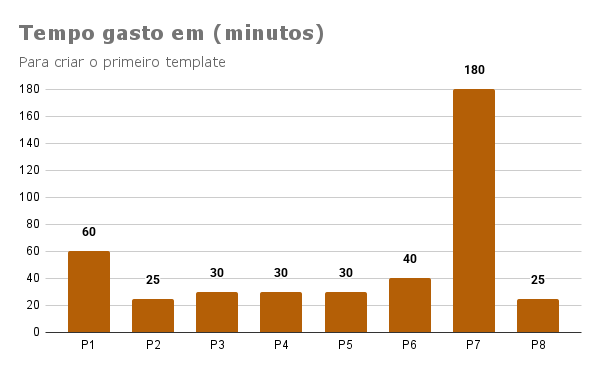
\includegraphics[width=16cm]{./imagens/capitulo8/tempo-gasto}
	\caption{Tempo médio de criação do primeiro template (Elaboração própria, 2025) }
	\label{fig:tempo-gasto}
\end{figure}
        \item \textbf{Numero de questões geradas por template} : quantidade total de instâncias de questões produzidas a partir de um único template, considerando as combinações válidas de variáveis, quanto maior o repertório de questões geradas maior o poder de generalização do template.
\begin{figure}[ht]
	\centering
	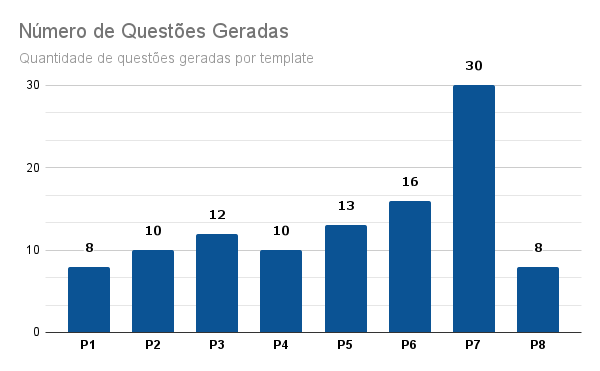
\includegraphics[width=16cm]{./imagens/capitulo8/questoes-geradas}
	\caption{Numero de questões geradas por template (Elaboração própria, 2025) }
	\label{fig:questoes-geradas}
\end{figure}
        \item  \textbf{Sucesso em converter a questão existente em template }: indica se foi possível ou não transformar uma questão existente em um template funcional, mantendo sua essência pedagógica, o questionário indicou que todos os participantes responderam "sim" para conversão de uma questão existente em template, com exceção de um. 
    \end{itemize}


\section{Resultados Observados}

Para além dos indicadores objetivos foi aplicado um bloco de afirmações em escala \textit{Likert} (5 = \textit{Concordo totalmente} .... 1 = \textit{Discordo totalmente})  para entender como os professores enxergam a abordagem. As figuras 1 2 e 3 sintetizam os resultados agrupados em três dimensões conforme a tabela 3.


\begin{table}[H]
    \centering
    \caption{Síntese comparativa das dimensões avaliadas na escala Likert (N = 8)}
    \label{tab:dimensoes-likert}
    \begin{tabular}{p{0.15\textwidth} p{0.40\textwidth} p{0.35\textwidth}}
        \toprule
        \textbf{Dimensão} & \textbf{Principais evidências levantadas} & \textbf{Implicação para as QPs}\\ \midrule
        Preferência de Uso &
        \begin{itemize}[leftmargin=*]
            \item \textbf{Adaptação}: 7 de 8 dos professores \textit{concordam} ou \textit{concordam totalmente} que preferem adaptar modelos prontos.%
            \item \textbf{Criação do zero}: 5 de 8 \textit{discordam} ou \textit{discordam totalmente} de criar tudo do zero.%
        \end{itemize} &
        Reforça a \textbf{viabilidade operacional} do repositório-base (QP1) e o potencial de \textbf{reutilização}. \\ \midrule
        
        Intenção de Uso &
        \begin{itemize}[leftmargin=*]
            \item 6 de 8 indicariam a ferramenta a colegas outros professores. Mas o uso na disciplina dividiu opiniões (4 neutras e 4 negativas)%
        \end{itemize} &
        Sinaliza \textbf{barreiras de adoção} que exigem suporte, necessita de uma adequação na abordagem. \\ \midrule
        
        Percepção de Utilidade &
        \begin{itemize}[leftmargin=*]
            \item todos compreenderam a estrutura dos templates.%
            \item Todos concordaram que o ChatGPT facilita muito as variações.%
            \item 4 de 8 professores julgaram a curva de aprendizagem longa.%
        \end{itemize} &
        a curva de aprendizagem evidencia um \textbf{custo inicial} (QP3), precisa de muito esforço cognitivo para o entendimento conceitual. \\ \bottomrule
    \end{tabular}
\end{table}



\begin{figure}[ht]
	\centering
	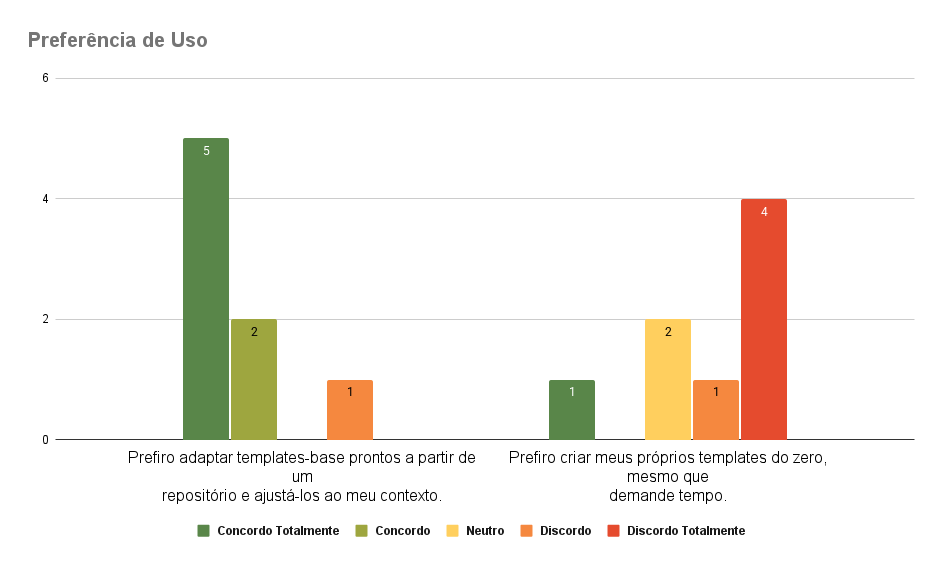
\includegraphics[width=16cm]{./imagens/capitulo8/preferencia-uso}
	\caption{Preferencia de uso  (Elaboração própria, 2025) }
	\label{fig:preferencia-uso}
\end{figure}


\begin{figure}[ht]
	\centering
	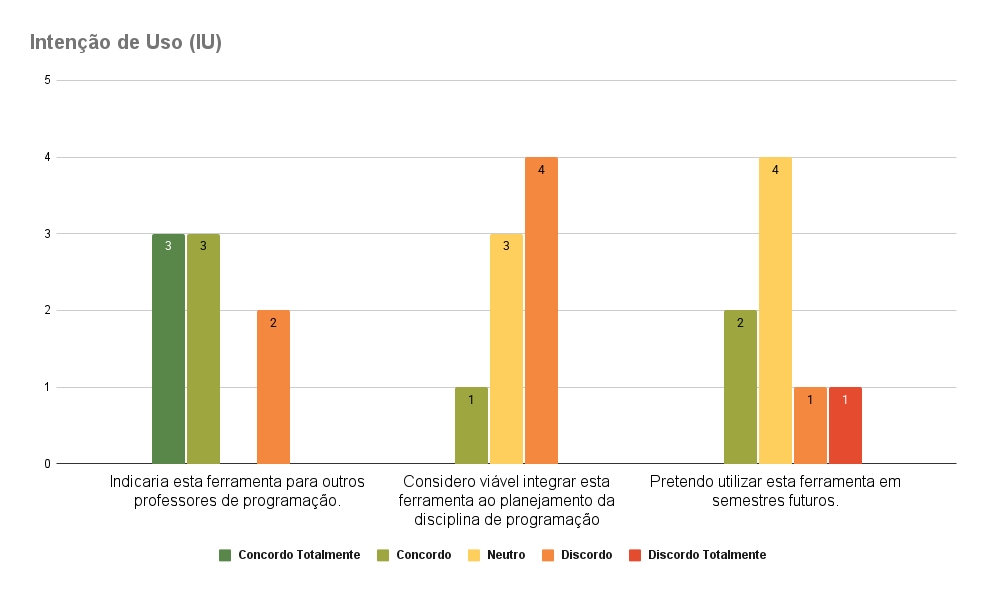
\includegraphics[width=16cm]{./imagens/capitulo8/intencao-uso}
	\caption{Intenção de uso  (Elaboração própria, 2025) }
	\label{fig:intencao-uso}
\end{figure}



\begin{figure}[ht]
	\centering
	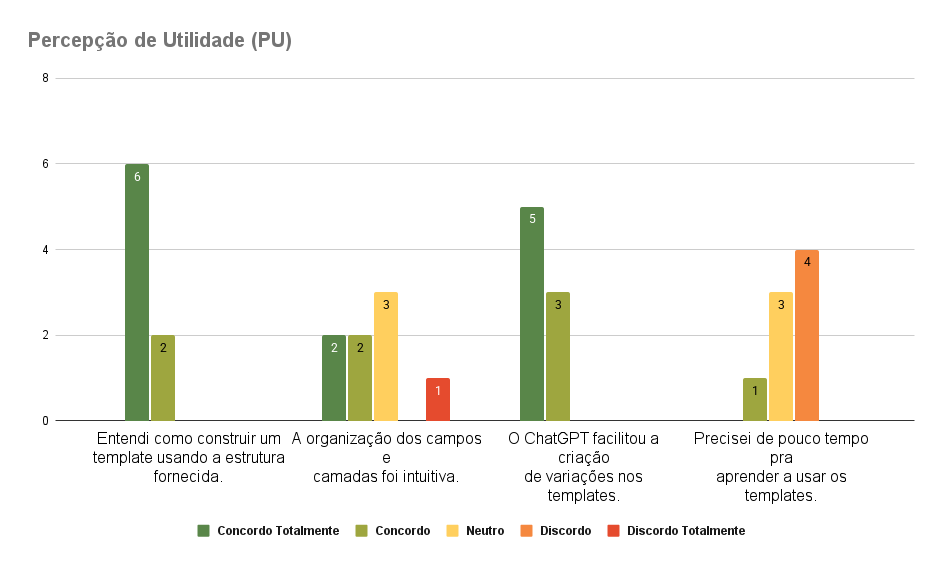
\includegraphics[width=16cm]{./imagens/capitulo8/percepcao-utilidade}
	\caption{Percepção de utilidade  (Elaboração própria, 2025) }
	\label{fig:percepcao-utilidade}
\end{figure}

	
\section{Relatos de respostas abertas}


Os comentários e sugestões abertos reforçam e contextualizam os achados quantitativos (vide Figura~\ref{fig:dificuldades-encontradas}).  Embora a \textit{Estruturação das ramificações} apareça como a dificuldade mais frequente (8 menções), os relatos mostram que o problema não se restringe à lógica condicional em si, mas se estende à **carga cognitiva exigida para “visualizar” o fluxo de um template multicamadas apenas a partir de texto JSON**.

\begin{table}[H]
\centering
\caption{Síntese dos relatos abertos (N~=~7)}
\label{tab:relatos-abertos}
\begin{tabular}{p{0.24\textwidth} p{0.28\textwidth} p{0.28\textwidth} p{0.14\textwidth}}
\toprule
\textbf{Categoria} & \textbf{Principais evidências} & \textbf{Necessidades/sugestões} & \textbf{Freq.}\\ \midrule
\textbf{Desafios cognitivos} & \begin{itemize}[leftmargin=*]
    \item “Exige muita abstração” \newline
    \item “Difícil enxergar o template usando JSON”
\end{itemize} & Visualização em camadas; exemplos guiados & 5 \\ \midrule
\textbf{Curva de aprendizagem} & \begin{itemize}[leftmargin=*]
    \item “Curva de aprendizado é uma limitação” \newline
    \item Dependência do ChatGPT para começar
\end{itemize} & Repositório de modelos-base; tutoriais passo a passo & 6 \\ \midrule
\textbf{Manipulação de JSON} & \begin{itemize}[leftmargin=*]
    \item “Difícil manipular texto JSON” \newline
    \item Erros de sintaxe e concordância
\end{itemize} & Editor visual + validador automático & 4 \\ \midrule
\textbf{Tempo de elaboração} & \begin{itemize}[leftmargin=*]
    \item “Tempo gasto em pensar no formato é alto” 
\end{itemize} & Assistente de pré-visualização e depuração & 3 \\ \midrule
\textbf{Benefícios percebidos} & \begin{itemize}[leftmargin=*]
    \item “A ideia é boa” \newline
    \item “ChatGPT facilitou muito”
\end{itemize} & Manter integração com IA; ampliar exemplos & 2 \\ \bottomrule
\end{tabular}
\end{table}

\paragraph{Principais barreiras.}
Os docentes relatam quatro obstáculos centrais:

\begin{enumerate}[label=(\alph*)]
    \item \textbf{Visualização da lógica}: a ausência de uma representação gráfica torna difícil acompanhar onde cada variável é injetada e como as ramificações se desdobram.
    \item \textbf{Falta de modelos-base}: professores novatos no método sentem‐se “sem chão” para iniciar, o que tornou a \emph{Falta de modelos-base prontos} a terceira dificuldade mais citada (4 menções).
    \item \textbf{Sintaxe JSON}: erros simples (vírgulas, chaves) quebram o template inteiro; isso desestimula a exploração manual.
    \item \textbf{Tempo e dependência de IA}: ainda que o ChatGPT acelere o processo, há receio de enviesar o template ou de introduzir erros de concordância.
\end{enumerate}

\paragraph{Sugestões de melhoria.}
Quase todos os participantes convergiram em três frentes:

\begin{enumerate}[label=(\roman*)]
    \item **Interface gráfica em blocos** que permita “arrastar e soltar” condições e variáveis, reduzindo a necessidade de editar JSON cru.
    \item **Pré-visualizador dinâmico** para executar combinações e verificar, em tempo real, a coerência dos enunciados gerados.
    \item **Repositório de templates prontos**, organizado por assunto e nível de dificuldade, servindo como ponto de partida e material de estudo.
\end{enumerate}

\paragraph{Implicações para as Questões de Pesquisa.}
Os relatos revelam que, apesar da alta viabilidade operacional indicada pelos indicadores objetivos, a adoção em larga escala depende de \emph{ferramentas de suporte à autoria}.  Endereçar as três frentes acima pode:

\begin{itemize}
    \item Reduzir o tempo médio de criação de templates (\textbf{QP2});
    \item Aumentar a taxa de reaproveitamento, pois modelos bem estruturados tendem a ser compartilhados (\textbf{QP3});
    \item Mitigar a principal limitação já identificada em QP1—o esforço cognitivo para estruturar ramificações.
\end{itemize}

\begin{figure}[ht]
	\centering
	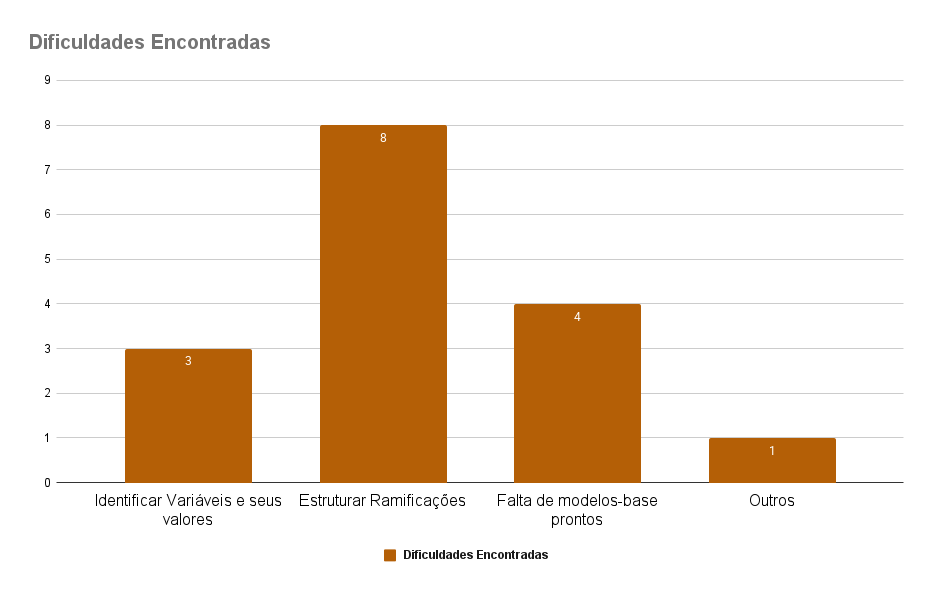
\includegraphics[width=16cm]{./imagens/capitulo8/dificuldades-encontradas}
	\caption{Dificuldades encontradas  (Elaboração própria, 2025) }
	\label{fig:dificuldades-encontradas}
\end{figure}

	

\section{Benefícios e Desafios Percebidos}


O estudo revelou que os professores conseguiram elaborar templates funcionais e diversificados, utilizando as orientações fornecidas. No entanto, alguns desafios foram identificados:

\begin{enumerate}
    \item \textbf{Dificuldade Inicial}: Professores com menor familiaridade com conceitos de questões baseada em templates demonstraram dificuldades em identificar elementos variáveis e combinar os valores.
    \item \textbf{Uso da IA Gnerativa} : A integração do ChatGPT foi bem recebida, e os participantes relataram que as sugestões fornecidas pela ferramenta ajudaram na proposta de contextos diversificados.
    \item \textbf{Percepção Geral} : Os professores consideraram o modelo útil para reduzir o tempo de elaboração de questões, no entanto preferiram que os templates já estivessem prontos pra utilizar, e após construídos pudessem acrescentar ou editar a estrutura conforme a necessidade ao invés de criar do zero.
\end{enumerate}


\begin{table}
\centering

\begin{tabular}{l}
 \\

\end{tabular}

\end{table}

\begin{table}
\centering

\begin{tabular}{l}
\textbf{Resultados} \\

\end{tabular}

\end{table}

\begin{table}
\centering

\begin{tabular}{l}
Quantitativos (tabelas/gráficos) e qualitativos (depoimentos). \\

\end{tabular}

\end{table}

 
\section{Beneficios e Desafios Percebidos} 

redução do esfoço de elaboração, maior diversidade de exercicio

identificar corretamente as variaveis e seus valores
curva de aprendizagem para manipular o template
preferencia em usar templates-base prontos em vez de começar do zero.

\section{Considerações Finais do Estudo de Caso}
A aplicação foi realizada com um número reduzido de professores, o que limita a generalização dos resultados. Estudos futuros poderão expandir o alcance para incluir mais participantes para validar a proposta. Apesar das limitações, a abordagem de geração automática de questões demonstrou um potencial significativo para criar questões em escala e reduzir o esforço necessário para a construção de conteúdos por parte dos professores.


RESPOSTA AS QUESTÕES DE PESQUISA COM OS INDICADORES 
VIABILIDADE : INDICADOR DE TEMPO
UTILIDADE : TAXA DE APROVEITAMENTO 
DESAFIOS : FALTA DE MODELOS PRÉ-PRONTOS

AMOSTRA REDUZIDA LIMITA A GENERALIZAÇÃO

----- CONTINUE AQUOI ---  PARE AQUIIII


\subsubsection{\textbf{Resultados}}

\paragraph{\textbf{7.8.1 Eficiência do processo}}

Tempo médio para criar o primeiro template: 27 min (desvio-padrão 6,2 min). Média de 12,4 questões por template e reaproveitamento de 83 \%.

\paragraph{\textbf{7.8.2 Depoimentos dos professores}}

\begin{quote}
“Com o guia, consegui transformar rapidamente uma questão antiga em um template; a IA me ajudou a criar três variações de contexto em minutos.” — P2

\end{quote}

\paragraph{\textbf{7.8.3 Benefícios percebidos}}

Redução do esforço de elaboração, maior diversidade de exercícios e incremento no engajamento dos alunos.

\paragraph{\textbf{7.8.4 Desafios e dificuldades}}

\begin{itemize}
    \item Identificar corretamente as variáveis e seus valores.
    \item Curva de aprendizagem para manipular placeholders.
    \item Preferência por templates-base prontos em vez de começar do zero.
\end{itemize}
 

\paragraph{\textbf{Principais Desafios Identificados}}

\begin{itemize}
    \item \textbf{Curva de aprendizagem inicial} (especialmente na identificação de variáveis e condições);
    \item \textbf{Necessidade de modelos‐base} para acelerar a adoção;
    \item \textbf{Integração com sistemas de avaliação existentes} (Moodle, Google Forms, etc.), que exigirá conversores automáticos — apontado como trabalho futuro.
\end{itemize}
\textbf{QP3 – Desafios:} maior dificuldade em definir variáveis e preferências por templates‐base prontos; 60 \% solicitaram um repositório inicial de modelos. 


Síntese interpretativa
Em conjunto, os três gráficos indicam que:

Viabilidade: a mediana de ~30 min coloca a criação de templates dentro de um tempo aceitável para reuniões de planejamento.

Eficiência: gerar entre 10 e 15 questões a partir de um único template demonstra economia de esforço na produção de exercícios.

Reutilização: a taxa de sucesso plena na conversão de questões reais comprova que o método não exige partir do zero, favorecendo adoção incremental.